%
% Chapter 8
%

\chapter{BACKGROUND PREDICTIONS}
Despite optimizing the event selection criteria to select signal events, a substantial amount of background events from a variety of processes enter the signal region.
These backrounds are classified as being either reducible or irreducible, and are estimated differently depending on this classification. An understanding
of each background process and a proper assessment of the uncertainity associated with the estimation of each background is critical to extracting the signal and interpreting
the results. 

\section{Reducible backgrounds}
Reducible backgrounds arise from a number of sources, but always contain leptons that are either non-prompt, or have a lepton whose electric charge is mismeasured.
Reducible backgrounds are estimated from data-driven approaches using control regions and extrapolation techniques to predict their contribution to the yield in the
signal region. 
These backgrounds are classified as reducible because if the event selection and CMS object reconstruction worked with perfect efficiency, the events would not
enter the signal region, thus improving the prompt lepton identifiction and CMS lepton electric charge measurement can reduce the contributions from these processes.
The background due to fakes is entirely separate from the charge mismeasurement background and are estimated separately. 

\subsection{Fake lepton background} 
The fake lepton background gets its name from the fact that events with non-prompt leptons pass the tight selection and enter the signal region by faking prompt leptons. These
fakes, or non-prompt leptons, typically originate from hadronic decays of jets, and with the primary source of this being the relatively large cross-section semi-leptonic \ttbar
process, where the b-jet from the leptonic top quark produces a fake lepton that passes the tight lepton selection criteria, but also includes other processes where a lepton
is produced inside a jet. The background from these events is estimated via a loose-to-tight extrapolation. This begins with measuring the rate at which the leptons passing
the fakeable selection also pass the tight selection. The measurement is performed in a control region with data.
The measurement is then used to extrapolate from a sideband with fakeable leptons to the signal region with
tight leptons to estimate the signal region contribution from to events with fake leptons. 

A control region heavily enriched in QCD multijet events is designed to measure the probability of a non-prompt lepton passing the fakeable selection to also pass the tight selection.
This probability is called the fake rate, and the control region is referred to as the measurement region. The measurement region requires events with one loose lepton and one
hadronic jet isolated from the lepton with $\Deta$R $\gt$ 0.7. This selection enriches the measurement region with non-prompt leptons. The data analyzed in the measurement region is collected on single lepton
triggers which require a single lepton and a particle-flow jet with \pt $\gt$ 30 GeV.

Because the lepton \pt threshold in the signal region (25,15 GeV) is lower than the trigger threshold (30 GeV) in the fake rate measurement region,
the fakeable definition must not depend on whether or not the lepton passed the trigger to avoid biasing the fake rate measurement. To achieve this, we introduce the ``corrected'' \pt, which is the
same as the standard \pt if the lepton passes the tight selection, but modified to 0.9 times the nearest jet \pt otherwise. The trigger bias has been explicitly checked in lepton-enriched QCD MC events, 
where the fake rate is studied with and without requiring the lepton to pass the trigger. This study showed that the trigger turn-on curve requires the trigger \pt threshold to be significantly lower than
the corrected \pt to avoid any bias. Thus the triggers used to collect the data in the measurment region are as loose as \textsc{HLT$\_$Mu3$\_$PFJet40}, \textsc{HLT$\_$Mu8}, and \textsc{HLT$\_$Ele8$\_$XX}
 which allows for corrected \pt to be as low as 14 GeV.
This motivates the choice of corrected \pt cut of 15 GeV on the subleading lepton in the signal region. 

To ensure a high purity of fake leptons in the measurement region, the contribution of prompt leptons must be accounted for. This contribution arises from W and Z plus jets processes, but also from \ttbar. The Z contamination
is addressed by vetoing events with more than one loose lepton. To W component is subtracted with a fit to the transverse mass of the lepton and missing energy, $M_{T}(l,E_{T}^{miss})$. A cut is first applied requiring
$M_{T}(l,E_{T}^{miss}) < $15 GeV, with the residual contamination subtracted in each \pt bin using W/Z +jet MC. 

Once the fake rate is measured in the measurement region, it is applied in a second control region, also enriched in fakes, denoted as the application region. The weighted yields in this region constitute the background due to
fake leptons in the signal region. As such, the application region is identical to the signal region, except that one of the two same-sign leptons must fail the tight lepton selection. The fake rate weights are expressed
in terms of event yields as a function of the number of leptons failing the tight selection in a given event. The contribution of fakes in the signal region is calculated as:

\begin{equation}
\label{eqn:fake_rate}
  N_{pp}^{bkg} = \frac{f_{1}}{1-f_{1}}N_{pf} + \frac{f_{2}}{1-f_{2}}N_{pf} - \frac{f_{1}f_{2}}{(1-f_{1})(1-f_{2})}N_{ff}
\end{equation}

\noindent under the assumption that the contribution of prompt leptons failing the tight selection is negligible with respect to the number of non-prompt leptons failing. Here, $N_{pp}^{bkg}$ is the background contribution from fake leptons
in the signal region. $f_{1,2}$ is the fake rate for the leading, subleading lepton calculated from the measurement region, $N_{pf}$ is the number of events in the application region with 1 prompt and 1 fake lepton, and $N_{ff}$ is the
number of events in the application region with two fake leptons. 

Additional requirements to ensure closure with \ttbar MC  

\subsection{Charge mismeasurment background}

\section{Irreducible backgrounds}
Irreducible backgrounds are estimated strictly from MC. Irreducible backgrounds earn their name from the fact that even if the signal region and CMS event/object reconstruction
worked with perfect efficiency, they still contain the necessary objects to consistently pass the signal region selection and are thus irreducible with resepect to the signal
region definition. The dominant irreducible background processes include \ttw and \ttz. Other irreducible background processes include diboson pairs produced in association with jets,
while smaller contributions include processes with a single W or Z boson, a single top quark, tribosons, as well as other rare\footnote{Rare means a very small cross section, and very
small background contribution} SM backrounds. The modelling of these background processes has been checked to ensure a good agreement among the variable used to event selection and
signal extraction.  


%% \begin{figure}[hbtp]
%%  \begin{center}
%%    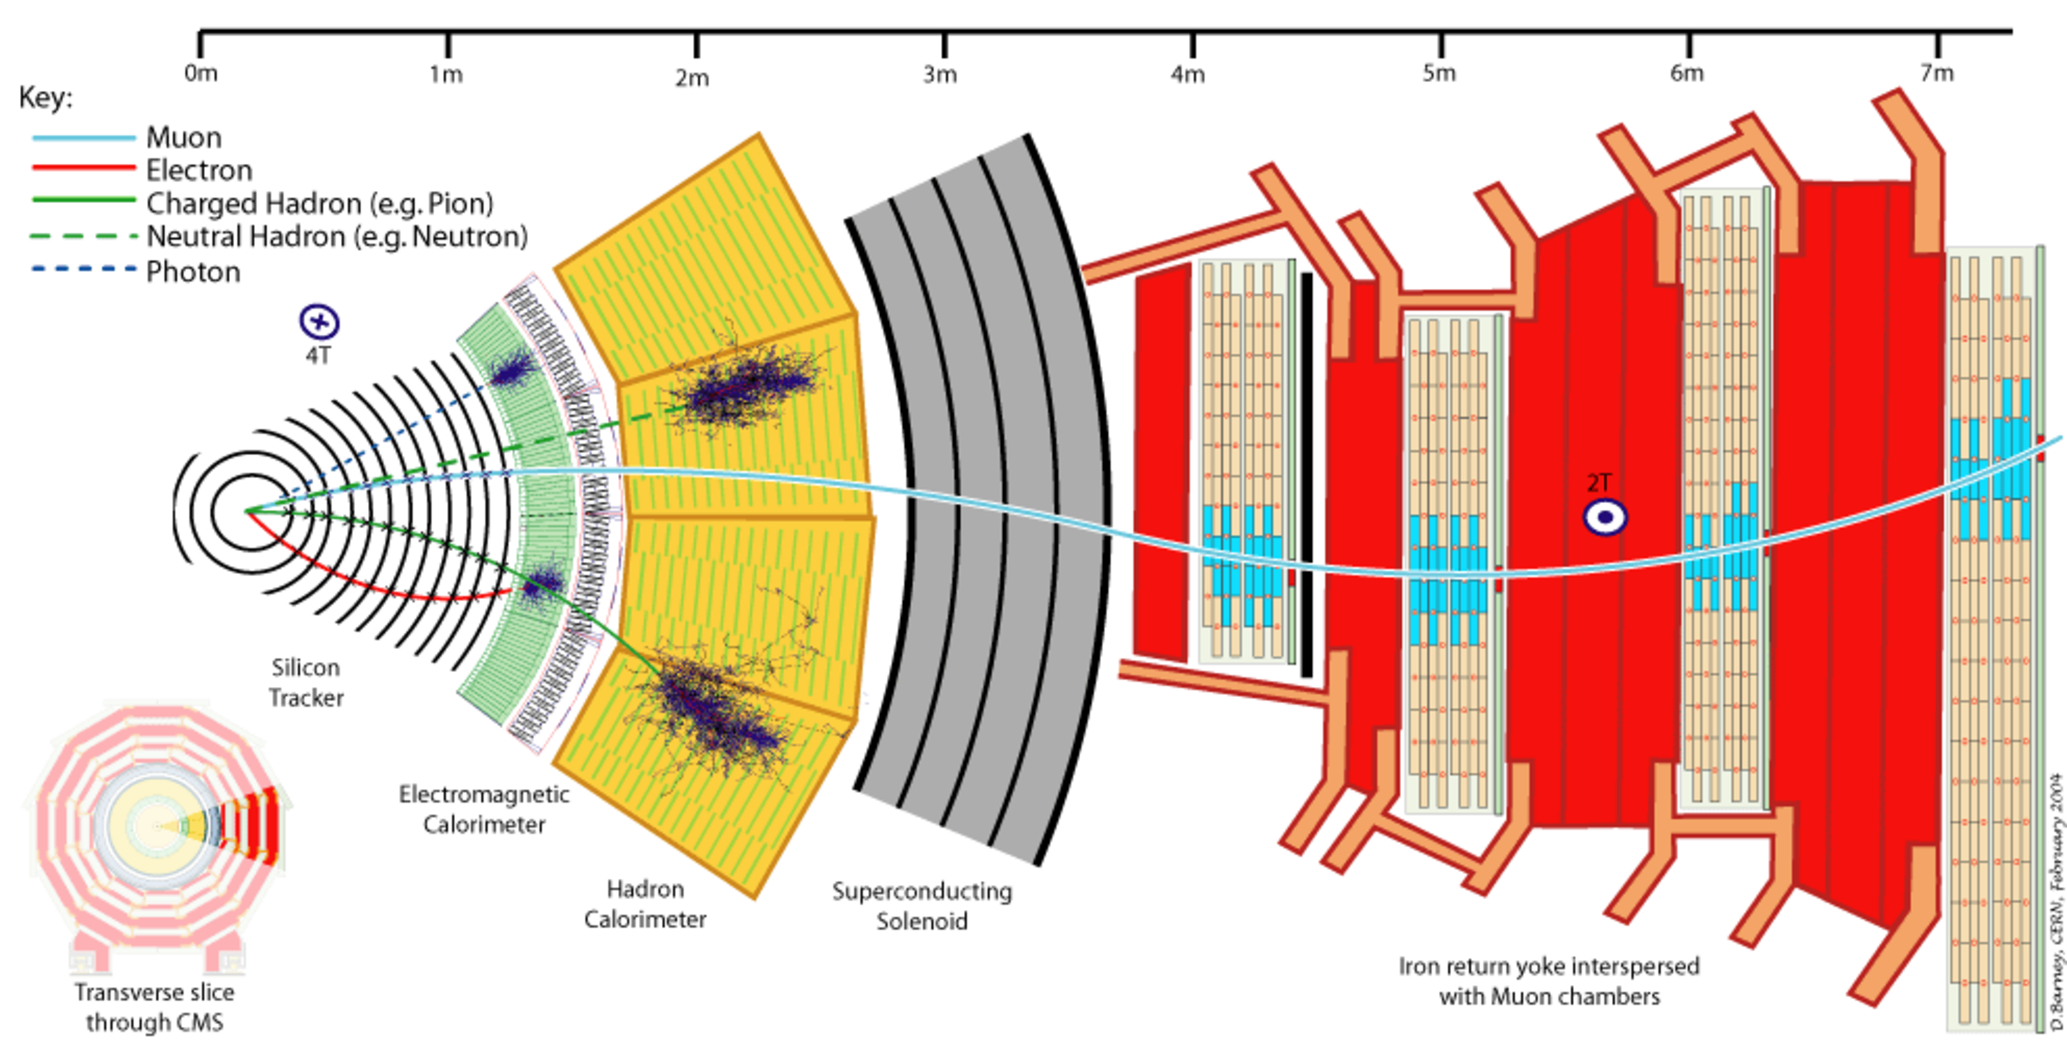
\includegraphics[width=0.8\textwidth]{ch4_figs/cms_particleflow.pdf}
%%    \caption{An overview of how CMS detects different types of particles. The slice of CMS in in the x-y plane.~\cite{NEED CITATION}.}
%%    \label{fig:cms_pflow}
%%  \end{center}
%% \end{figure}
